\section{Introduction}
Integrating the utilization of program analysis (PA) tools early in the development process of modern, large-scale software systems is crucial in determining the weaknesses/vulnerabilities in the code. Consider, for instance, a scenario in which a developer wants to use an online question and answering (Q\&A) forum, e.g., StackOverflow (S/O), to learn how to use software libraries or frameworks. Typically, the answer to a posed question comes as a fragment/chunk of code, which later makes it to the production application, stemming from the copy-and-paste software reuse practice. Unfortunately, if the copied code fragment is vulnerable, i.e., possesses defects that one can potentially exploit, it will result in the application being prone to attacks. Verdi {\em et al.}~\cite{verdi-tse22}
reviewed more than 72K C++ code snippets that migrated from 1,325 S/O answers, reporting a total of 99 vulnerable code snippets of 31 different types that made their way to 2,589 GitHub repositories.

Security researchers have proposed several automated approaches for
vulnerability detection using~program
analysis \cite{FlawFinder,RATS,viega2000its4,Checkmarx,HPFortify,Coverity,BufferOverFlow,SQLInj,Cross-siteScripting,AuthBypassSpoofing},
as well as machine learning (ML) and deep learning
(DL)~\cite{fse21,chakraborty2020deep,zhou2019devign,li2018sysevr,li2018vuldeepecker}
techniques. They leverage program representations such as
abstract syntax tree (AST), program dependence graph
(PDG)~\cite{fse21,li2018vuldeepecker}, control-flow graph
(CFG)~\cite{zhou2019devign}, data-flow graph
(DFG)~\cite{zhou2019devign}, code property graph
(CPG)~\cite{chakraborty2020deep}, etc., resulting from precise
automated analysis of software. However, extending such analyses to
code snippets is not straightforward as they are often incomplete,
unparseable, contain declaration/reference ambiguity, and are
interspersed between user comments. Currently, there exist tools such
as PPA~\cite{ppa08}, which parse an incomplete code fragment to build
the AST and extract data types in a best-effort manner, while
StaType~\cite{icse18} resolves the libraries and recovers only the
fully-qualified names for references.~However, the basic supports for
partial program analysis, i.e., for analyzing incomplete code are not
yet available.
%Such an infrastructure must include fundamental supports/services at the structural, semantic, and execution levels, thus enabling the static and dynamic analysis techniques to be built upon. 
%Let us refer to this as \textit{partial program analysis infrastructure}.

In addition to vulnerability detection, such an 
%partial program analysis infrastructure 
infrastructure
is also beneficial to other software engineering (SE) tasks that can tolerate a low level of errors and imprecision in building program representations. For example, consider code completion~\cite{codefill-icse22,facebook-icse21}, in which a model provides suggestions to complete partial code. Existing state-of-the-art ML/DL-based code completion models are just based on the code sequences or utilize the syntactic structure in ASTs, but none leverage the program dependencies due to the nature of partial code. Next, consider the task of analyzing the code fragments in a bug report to connect it to the relevant source files for bug localization purposes~\cite{euler-fse19,icpc17}. Here too, a need for partial program analysis, specifically partial program dependence analysis, can be observed.

The other facets of program analysis tools that need to be considered are their soundness and completeness. For example, static analysis tools are designed to detect errors that are valid for all possible executions, which often come at the cost of multiple approximations. As a result, such tools tend to overestimate, resulting in false positives. Next, consider the task of symbolic execution, which is limited by the path explosion problem that hinders its applicability to large-scale software systems. The effectiveness of such a symbolic execution engine can be improved by enhancing the symbolic constraints of the variables, and by guiding it to explore the right subset of symbolic states. 

%While the state-of-the-art research and practice has been well-established for the analysis of the entire programs, very little research and knowledge has been achieved for partial program analysis. 
To this effect, we set out to investigate and develop {\tool}, a {\em \underline{Neural} Network-Based \underline{P}rogram \underline{A}nalysis} infrastructure. We aim to establish {\bf a scientific foundation, novel methodologies, frameworks, models, and algorithmic solutions for neural program analysis}. {\tool} addresses two major issues in existing PA tools: (a) enables analysis of incomplete code fragments, i.e., partial program analysis; (b) empowers existing PA tools by making them more sound and complete (Figure~\ref{fig:arch}). {\tool} will allow the construction of efficient program analysis techniques for (partial) code on which downstream software engineering applications can be built.

%% Research Objectives
\subsection{Research Objectives}
While the state-of-the-art research and practice has been well-established for deriving control-flow and program dependencies for entire programs, there have been little to no advancements in conducting such a program dependence analysis for partial programs. In this proposal, we set out to investigate and develop {\tool}, a {\em \underline{Neural} Network-Based \underline{P}rogram \underline{D}ependence \underline{A}nalysis} infrastructure, that enables (partial) program dependence analysis. Besides, leveraging one such neural network-based approach will help gain a significant time markup in dependency discovery in contrast to traditional program analysis tools.


\begin{center}
    \begin{minipage}{33.5em}
    The key philosophy that drives our work is that {\em the dependence analysis of partial code can be learned from the dependence analysis for entire programs via the wealth of information obtained from ultra-large-scale, open-source software repositories}.
    \end{minipage}
\end{center}


We draw motivation for such a data-driven, learning-based approach from the following. First, ultra-large-scale software repositories, e.g. GitHub (7M+ projects) and SourceForge (700k+ projects) contain an enormous collection of programs. These repositories amount to 1B+ lines of code, 10M+ revision logs, and 3M+ issue reports. This wealth of knowledge is an excellent source for {\tool}. Hindle {\em et al.}~\cite{} have shown that code has high repetitiveness and predictability, and can be captured well by statistical models. Thus, we expect to build ML/DL models to learn from those repositories. Second, in an empirical study on the repetitiveness, containment, and composability of PDGs in open-source projects, the PI group~\cite{} reported that among 17.5M PDGs with 1.6B PDG subgraphs, 14.3\% of the PDGs have all of their subgraphs repeated across different projects. Furthermore, in 15.6\% of the PDGs, at least 90\% of their subgraphs are likely to have appeared before in other projects. Thus, {\tool} could learn from PDGs with complete program dependencies retrieved from existing code repositories and derive the dependencies for the (partial) code fragment under study. Broadly, such a partial program dependence analysis infrastructure is similar in spirit to neural network-based dependency parsing approaches in natural language processing (NLP), which learn the dependencies signifying the semantic relationships between words in a sentence from the text corpora.

We propose the following thrusts of research:

\vspace{3pt}
\noindent \textbf{[Thrust 1] Lorem}

\vspace{3pt}
\noindent \textbf{[Thrust 2] Neural Network-Based Program Dependence Analysis Infrastructure.} The basic infrastructure has two main tasks. First, it learns the well-defined syntactic and semantic information in source code by leveraging the program representations obtained for the complete programs in the training dataset, collected from large-scale code repositories. Next, one such trained model infers the program dependencies among the statements in any given code fragment, either complete or partial code.

\vspace{3pt}
\noindent \textbf{[Thrust 3] Enabling Fragment-Level Vulnerability Detection with \tool.} Vulnerability detection in code fragments can be facilitated as follows: (a) employing \tool infrastructure to predict the CFG/PDG for a given code fragment; (b) leveraging an existing automated VD tool that utilizes the predicted CFG/PDGs to identify the presence of vulnerabilities in partial code fragments.


%% Methodology and Anticipated Results
\subsection{Methodology and Anticipated Results}
\begin{itemize}
    \item {\bf Task A.} Collect high-quality, compilable Java and C/C++ programs and extract PDG/CFGs.
    \item {\bf Task B.} Design preliminary model to predict inter-statement control-flow and program dependencies.
    \item {\bf Task C.} Implement model and design experiments for both qualitative and quantitative evaluation.
    \item {\bf Task D.} Leverage automated vulnerability detection tool to identify vulnerable code fragments.
    \item {\bf Task E.} Model testing, tool release, and manuscript dissemination.
\end{itemize}

\begin{figure}[h]
    \centering
    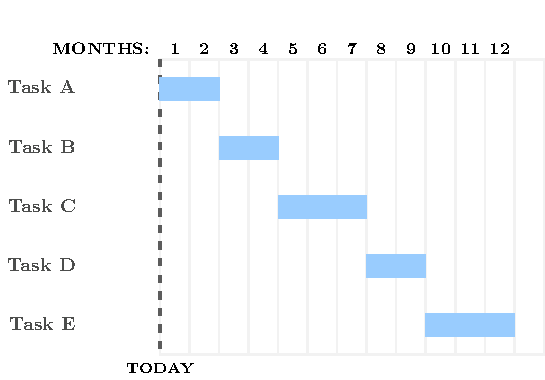
\includegraphics{gannt_charts/gannt.pdf}
    \caption{Anticipated Timeline}
    \label{fig:timeline}
\end{figure}

% Please add the following required packages to your document preamble:
% \usepackage[table,xcdraw]{xcolor}
% If you use beamer only pass "xcolor=table" option, i.e. \documentclass[xcolor=table]{beamer}
\begin{table}[]
\begin{tabular}{|ccc|}
\hline
\multicolumn{3}{|c|}{\cellcolor[HTML]{343434}{\color[HTML]{FFFFFF} \textbf{Project Milestones \& Deliverables}}}                                                                     \\ \hline\hline
\multicolumn{3}{|c|}{\textbf{T1. Benchmark Dataset Construction}}                                                                                                                    \\ \hline
\multicolumn{1}{|p{1cm}|}{\textbf{1.1}} & \multicolumn{1}{c|}{Collect high-quality, compilable Java and C/C++ programs and extract PDG/CFGs.}                           & Months 1 -- 2   \\ \hline\hline
\multicolumn{3}{|c|}{\textbf{T2. NeuralPDA Infrastructure}}                                                                                                                          \\ \hline
\multicolumn{1}{|p{1cm}|}{\textbf{2.1}} & \multicolumn{1}{c|}{Design and implement preliminary model to predict inter-statement control-flow and program dependencies.} & Months 3 -- 4   \\
\multicolumn{1}{|p{1cm}|}{\textbf{2.2}} & \multicolumn{1}{c|}{Enhance preliminary model and design experiments for both qualitative and quantitative evaluation.}       & Months 5 -- 7   \\ \hline\hline
\multicolumn{3}{|c|}{\textbf{T3. Fragment-Level Vulnerability Detection}}                                                                                                            \\ \hline
\multicolumn{1}{|p{1cm}|}{\textbf{3.1}} & \multicolumn{1}{c|}{Leverage automated vulnerability detection tool to identify vulnerable code fragments.}                   & Months 8 -- 9   \\
\multicolumn{1}{|p{1cm}|}{\textbf{3.2}} & \multicolumn{1}{c|}{Model testing, benchmark dataset and tool release, and manuscripts dissemination.}                        & Months 10 -- 12 \\ \hline
\end{tabular}
\end{table}

%% Preliminary Work
\subsection{Preliminary Work}
%Toward this theme, in our preliminary work, we developed DeepPDA, a neural network-based partial program dependence analysis approach that learns to derive the program dependencies for any code fragments (i.e., both complete and incomplete). In our preliminary empirical evaluation, we intrinsically evaluated it on Java and C/C++ programs. First, we trained {\tool} on complete code. For testing, we treated each method individually and chose a consecutive portion within the method to predict the program dependencies, and compared them against the actual dependencies. Overall, DeepPDA predicts CFG and PDG edges in Java with an F-score of 94.29\%, and in C++ with an F-score of 92.46\%.


In Figure~\ref{fig:model}, we present a preliminary design of the general architecture of \tool model. Given that attention is the driver behind the now ubiquitous Transformers’~\cite{Vaswani-2017} success in efficiently learning representations for different entities in different contexts, we plan to make it the foundation of the context learning components in our model as well. Each is intended to learn different aspects of contextualization. For our preliminary empirical evaluation, we collected Java methods from the GitHub Java Corpus~\cite{githubCorpus2013} and generated their CFG/PDGs using Joern program analysis tool~\cite{joern-2014}. By employing a self-attention network for both intra-statement and inter-statement contextualization, we trained a bootstrap model on complete code. For testing, we treated each method individually and chose a consecutive portion within the method to predict the program dependencies, and compared them against the actual dependencies. Overall, our bootstrap model was able to predict CFG and PDG edges in Java programs with an F-score of 94.29\%.



\section{Technical Merits}

\noindent \underline{{\bf Advance the state-of-the-art knowledge and
    understanding}}. Our research will fundamentally advance
the state-of-the-art research with novel theoretical foundations and
practical techniques in analyzing and building {\em program dependence
  graphs and program analysis, and vulnerability detection for partial
  code}.

\noindent \underline{{\bf Scientific foundation and creative/original
    research elements}}. We develop a scientific foundation, novel
methodologies, frameworks, models, and algorithmic solutions for
neural partial program analysis. Our infrastructure enpowers program
  analysis (PA) with advanced machine learning (ML) and artificial
  intelligence (AI) to enable the program analysis on incomplete code
  fragments.


